\documentclass{article}
\usepackage[utf8]{inputenc}
\usepackage{amsmath}
\usepackage{enumitem}
\usepackage{graphicx}
\usepackage{framed}
\usepackage{listings}
\usepackage{pdfpages}
\usepackage{caption}
\usepackage{subcaption}
\usepackage[utf8]{inputenc}
\usepackage{minted}
\usepackage{placeins}
\usepackage[utf8]{inputenc}
%\usepackage[english]{babel}
 
% \usepackage[
% backend=biber,
% style=alphabetic,
% sorting=ynt
% ]{biblatex}

\usepackage{natbib}
%\setcitestyle{authoryear,open={((},close={))}}
 
% \addbibresource{main.bib}


\title{Ch 11 Group}
\author{Tate Meehan, Arash Modaresi Rad, William Rudisill}
\date{March 2019}

\begin{document}
\maketitle

\section*{Equation}
The Van Genuchten equation is used to model volumetric soil water content as a function of pressure head: 
\begin{align}
\theta = \theta_r + \frac{\theta_s - \theta_r}{\big(1 + \alpha h^n\big)^m}
\end{align}


\section*{Part 1}
\subsection*{Part a}
The standard deviation for data is provided in Table 1 and is obtained form 10 soil samples with the same texture as the one used in this study. The "G" function can be found in the attached code. 


\begin{table}[]
\begin{tabular}{lll}
\hline
\multicolumn{3}{c}{Soil Code 1420}              \\ \hline
Preshead & Theta & \multicolumn{1}{c}{STD}      \\ \hline
10       & 0.52  & \multicolumn{1}{r}{0.044706} \\
50       & 0.505 & \multicolumn{1}{r}{0.042188} \\
100      & 0.47  & \multicolumn{1}{r}{0.030826} \\
204      & 0.42  & \multicolumn{1}{r}{0.019599} \\
340      & 0.38  & \multicolumn{1}{r}{0.020586} \\
680      & 0.33  & 0.033357                     \\
1033     & 0.3   & 0.029298                     \\
2067     & 0.27  & 0.040687                     \\
4858     & 0.24  & 0.034714                     \\
16540    & 0.19  & 0.040509                     \\ \hline
\end{tabular}
\end{table}


% \begin{table}[!h]
% \begin{center}
% \begin{tabular}{|c|c|c|c|c|c|}
% \hline
% & $\alpha = \mathbf{m_1}$ & $n = \mathbf{m_2}$ & $m = \mathbf{m_3}$ & $\theta_S = \mathbf{m_4}$ & $\theta_R = \mathbf{m_5}$ \\
% \hline
% Prior & .86 & .04 & .033 & 1.49 & .33 \\
% Recovered & .452 & .057 & .063 & 1.55 & .381 \\
% \hline
% \end{tabular}
% \caption{The prior and the recovered solution to the van Genuchten equation for a random starting guess.}
% \label{tab:2}
% \end{center}
% \end{table}




\subsection*{Part b}
We ran the MCMC code for 1e6 iteratons with a step size of .001 and a uniform prior distribution for the parameters. The accuracy rate was on the order of 10\%. Figure \ref{fig:2b} shows that the five parameters started with an autocorrelation of nearly one, which slowly deteriorated to near zero. 
\begin{figure}[!h]
    \centering
    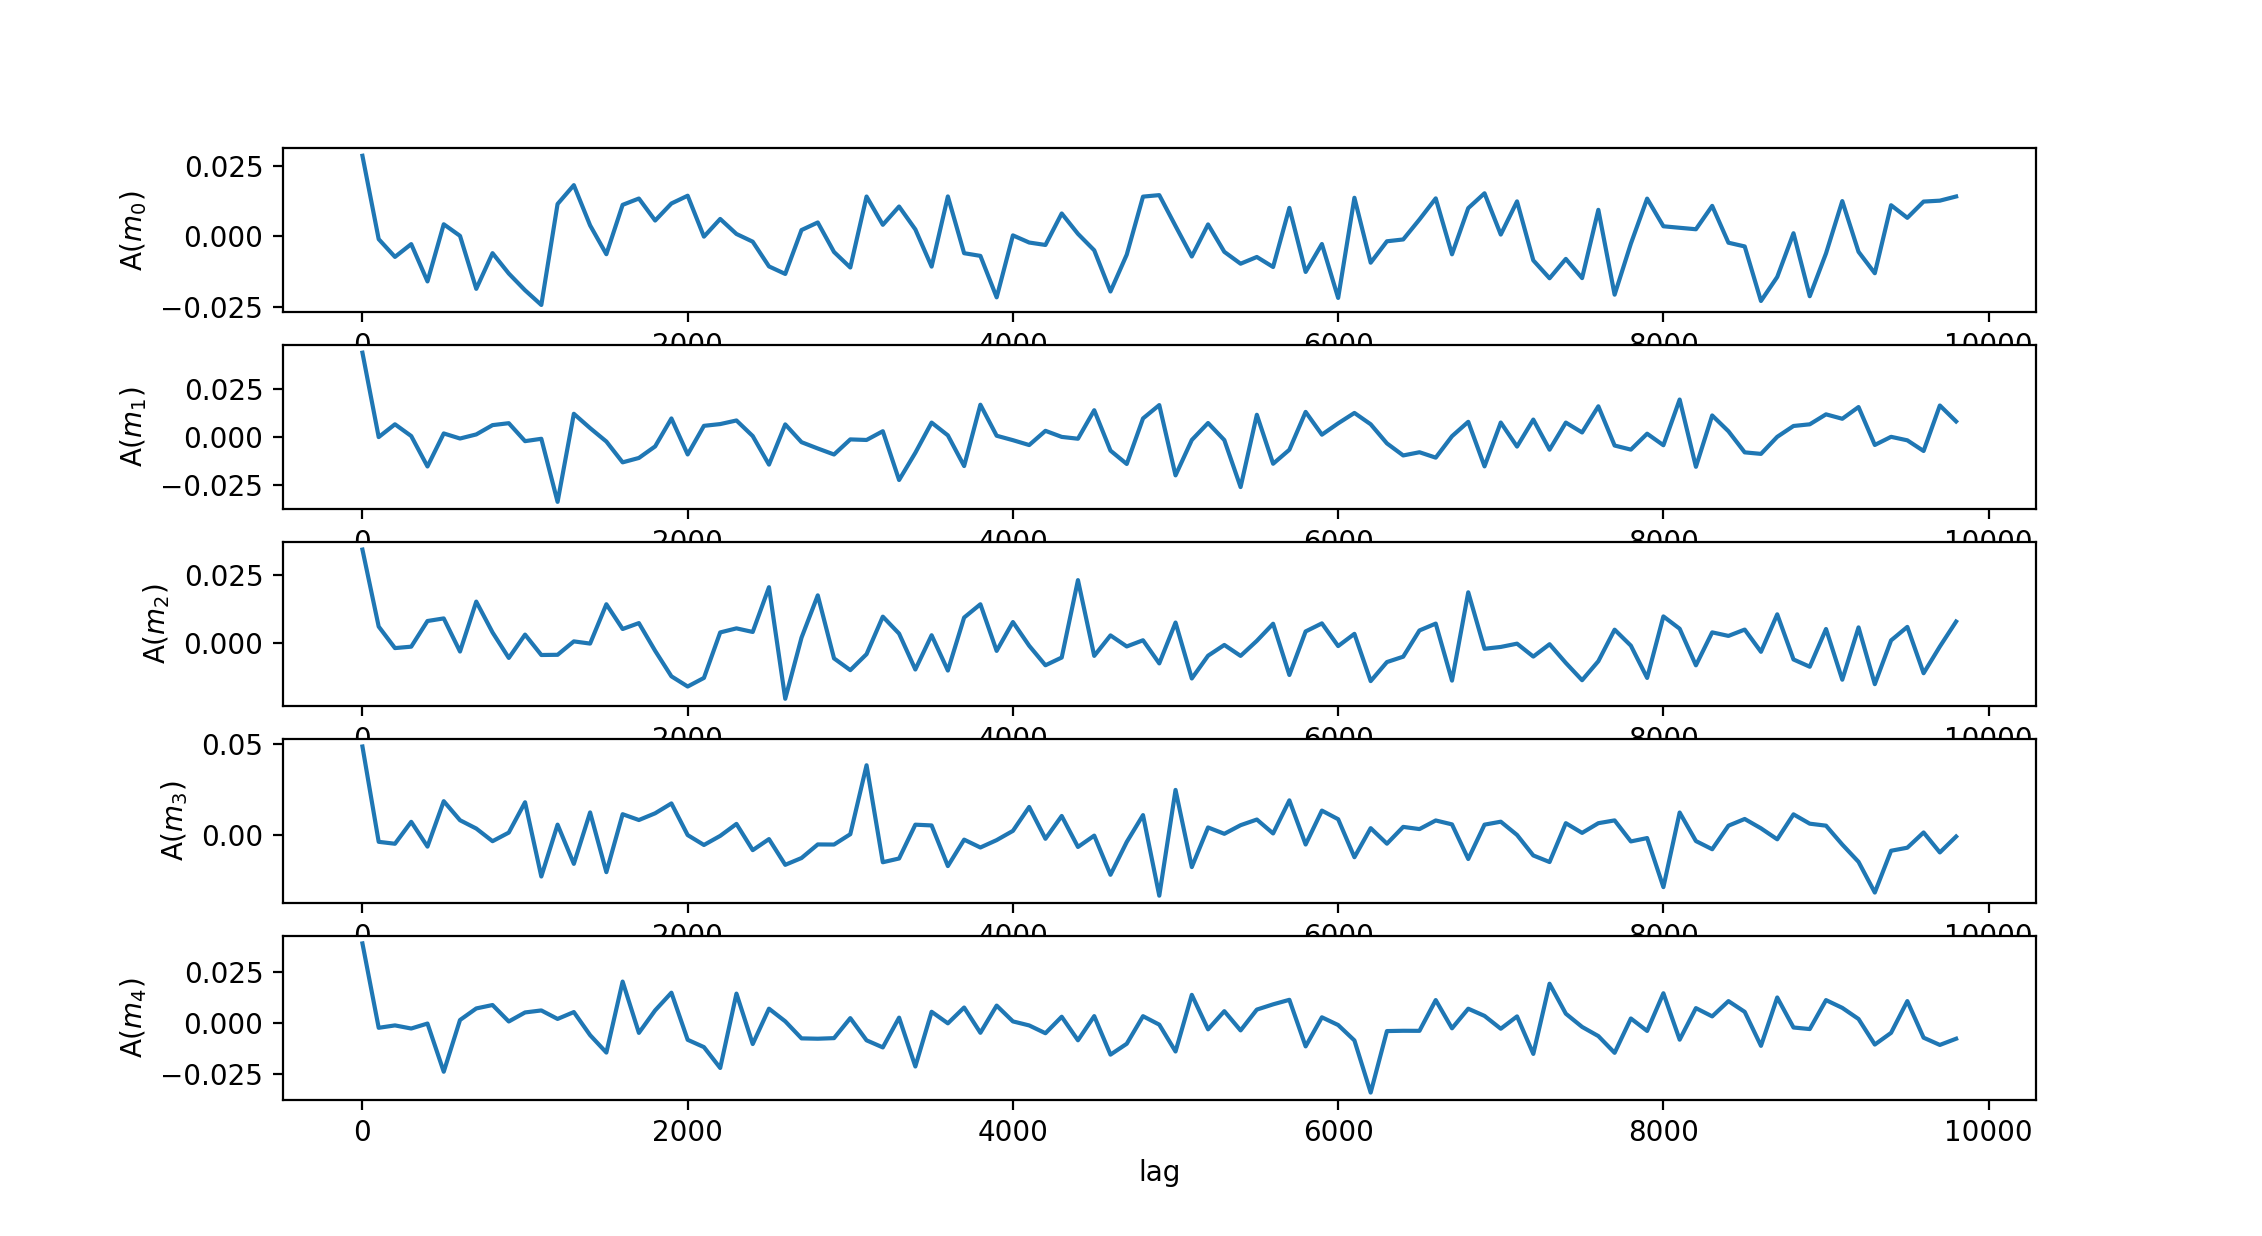
\includegraphics[width=\textwidth]{AutoCorr.png}
    \caption{Autocorrelations for posterior distribution parameters prior to thinning for autocorrelation reduction.}
    \label{fig:2b}
\end{figure}
From this we can conclude that a warm up of 100,000 steps would be appropriate in our case, since the parameters have a near zero auto-correlation. In fact, we could probably get away with an even lesser break-in period. The autocorrelation decays very quickly. 


\subsection*{Part C}
The MCMC history for a range of posterior samples are plotted in Figure \ref{fig:post_samples}. We selected 500 samples from the end of the MCMC iterations. There still appears to be some autocorrelation in the parameters. They are not entirely a 'white-noise' (uncorrelated) series; rather, the series appears to be more of a random-walk type series. 

\begin{figure}[!ht]
    \centering
    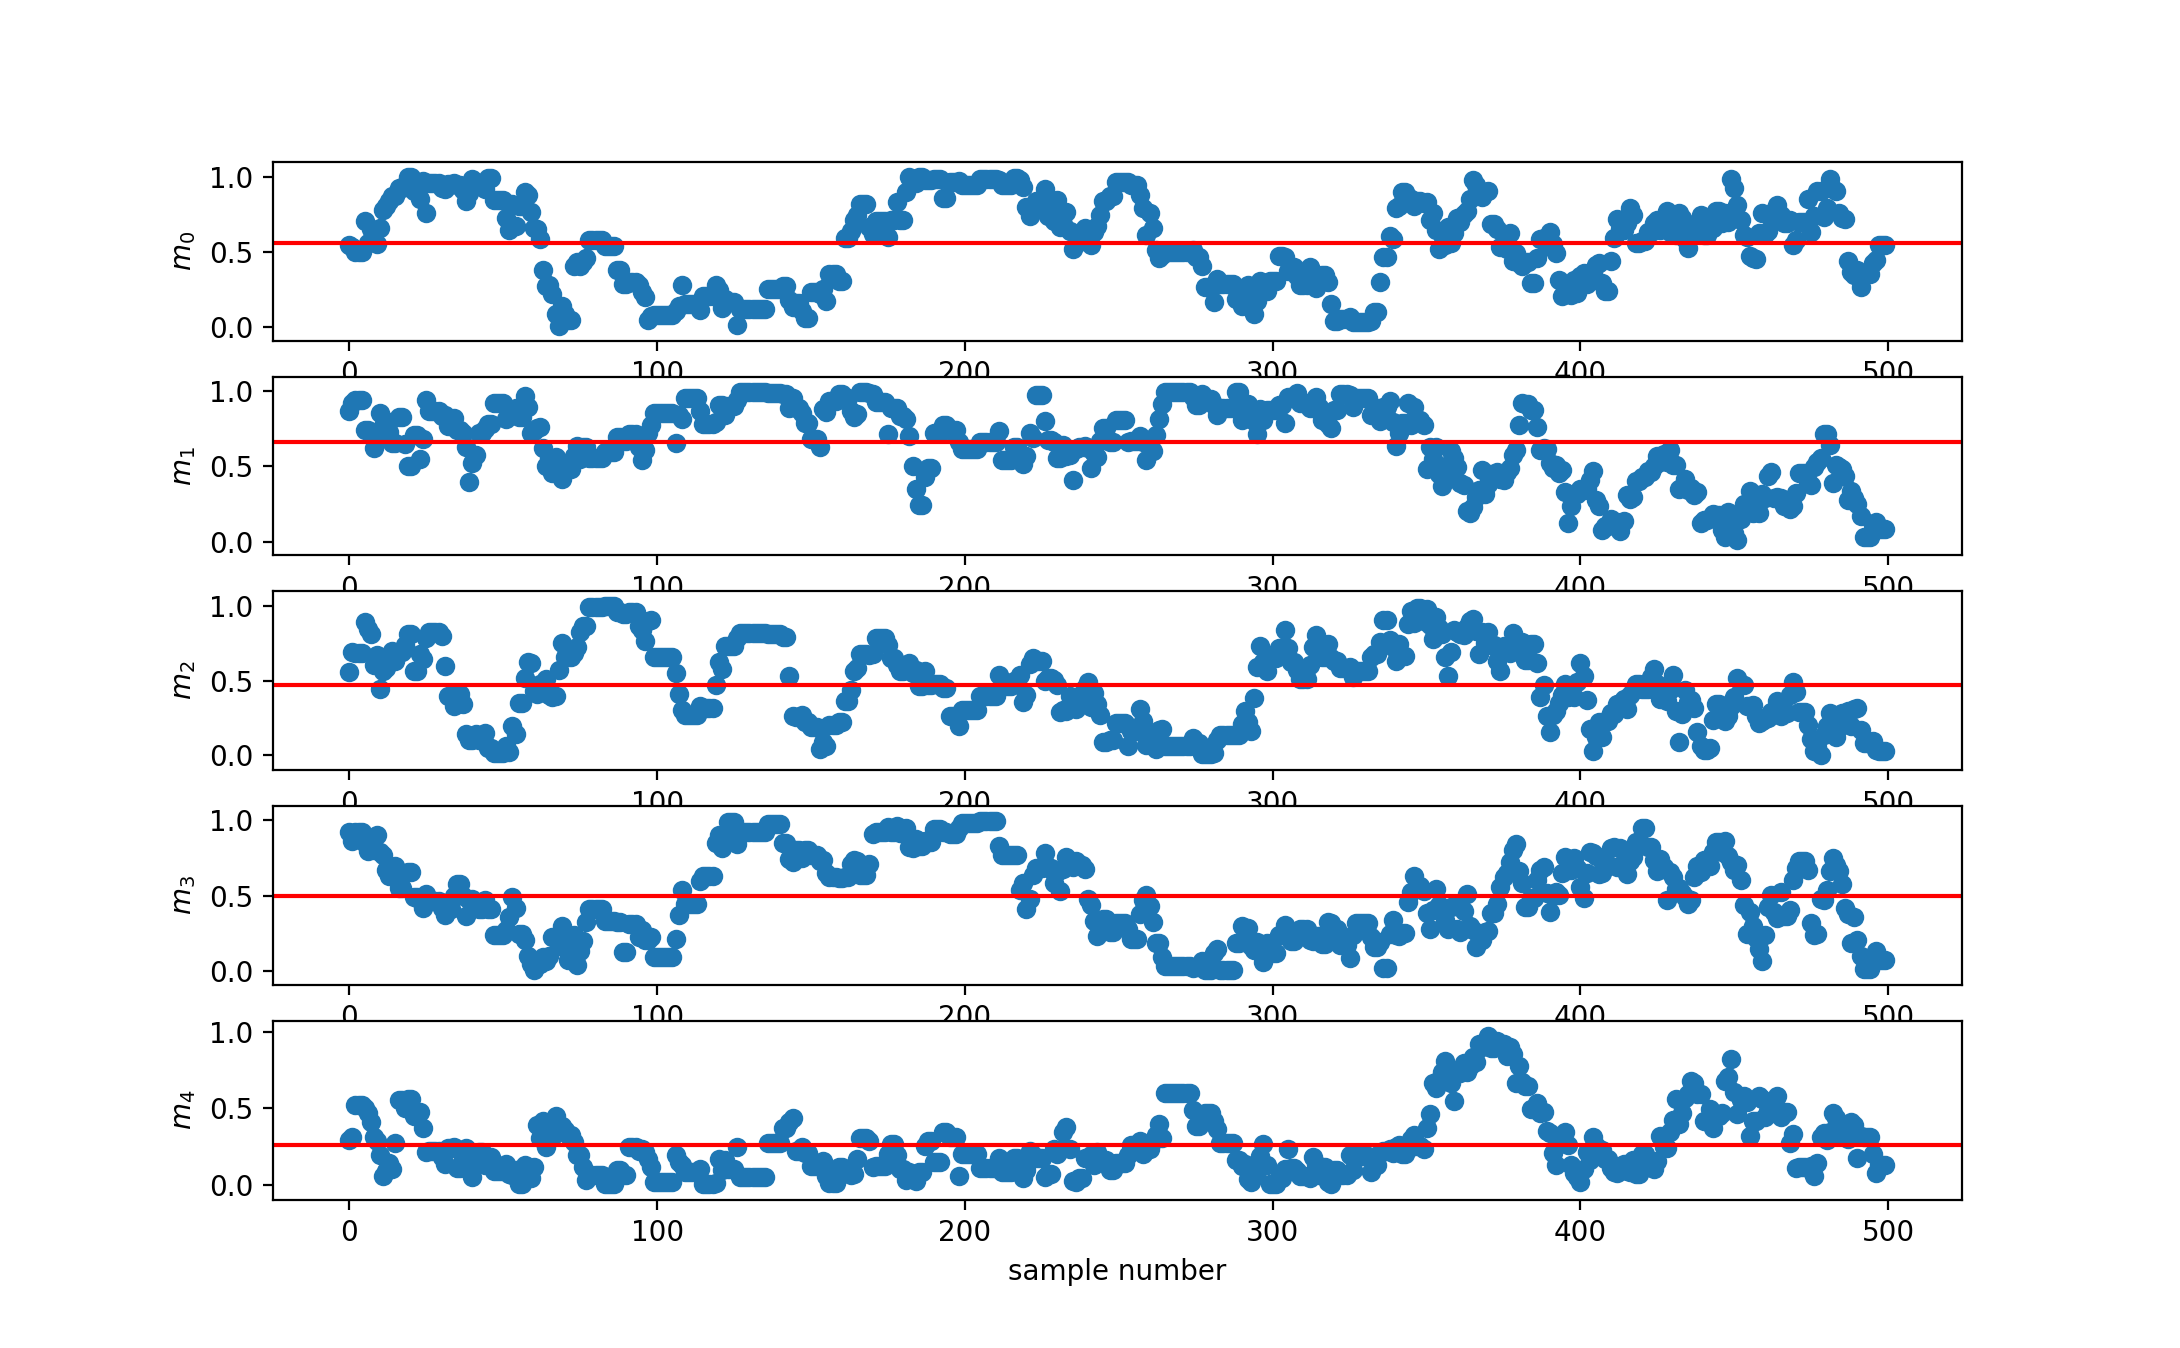
\includegraphics[width=4.5in]{part1_samples.png}
    \caption{MCMC History of posterior samples. The red line is the mean, not the true parameter estimate as it is in the book example}
    \label{fig:post_samples}
\end{figure}

\FloatBarrier

\subsection*{Part D}
Based on the histograms and scatter plots of the resulting sampled posterior distribution shown in Figure \ref{p1_post_dist}, it can be seen that our parameters estimates of MAP solution and also True model both do lay inside the 95\% probability intervals for every single parameter direction. Being inside the confidence intervals indicates that we have enclose well to the true solution. 
Despite that most histograms of the resulting sampled posterior distribution are somewhat close to having a uniform distribution. Notably, parameters 1 and 5 have approximately one-sided exponential distributions. The other parameters are much closer to a uniform distribution. It is possible that after more samples that these parameters would follow a uniform distribution. In our case this was a well-posed parameter estimation problem since in several runs of the MCMC we did not found different solutions with comparable likelihoods and we obtained the same solution every time indicating that this was a well-posed solution. The parameters are largely uncorrelated-- the scatter plots between the parameters do not show obvious correlations between parameter pairs. For comments about the well-posedness of the problem, refer to part 2 d. 


\begin{figure}[!ht]
    \centering
    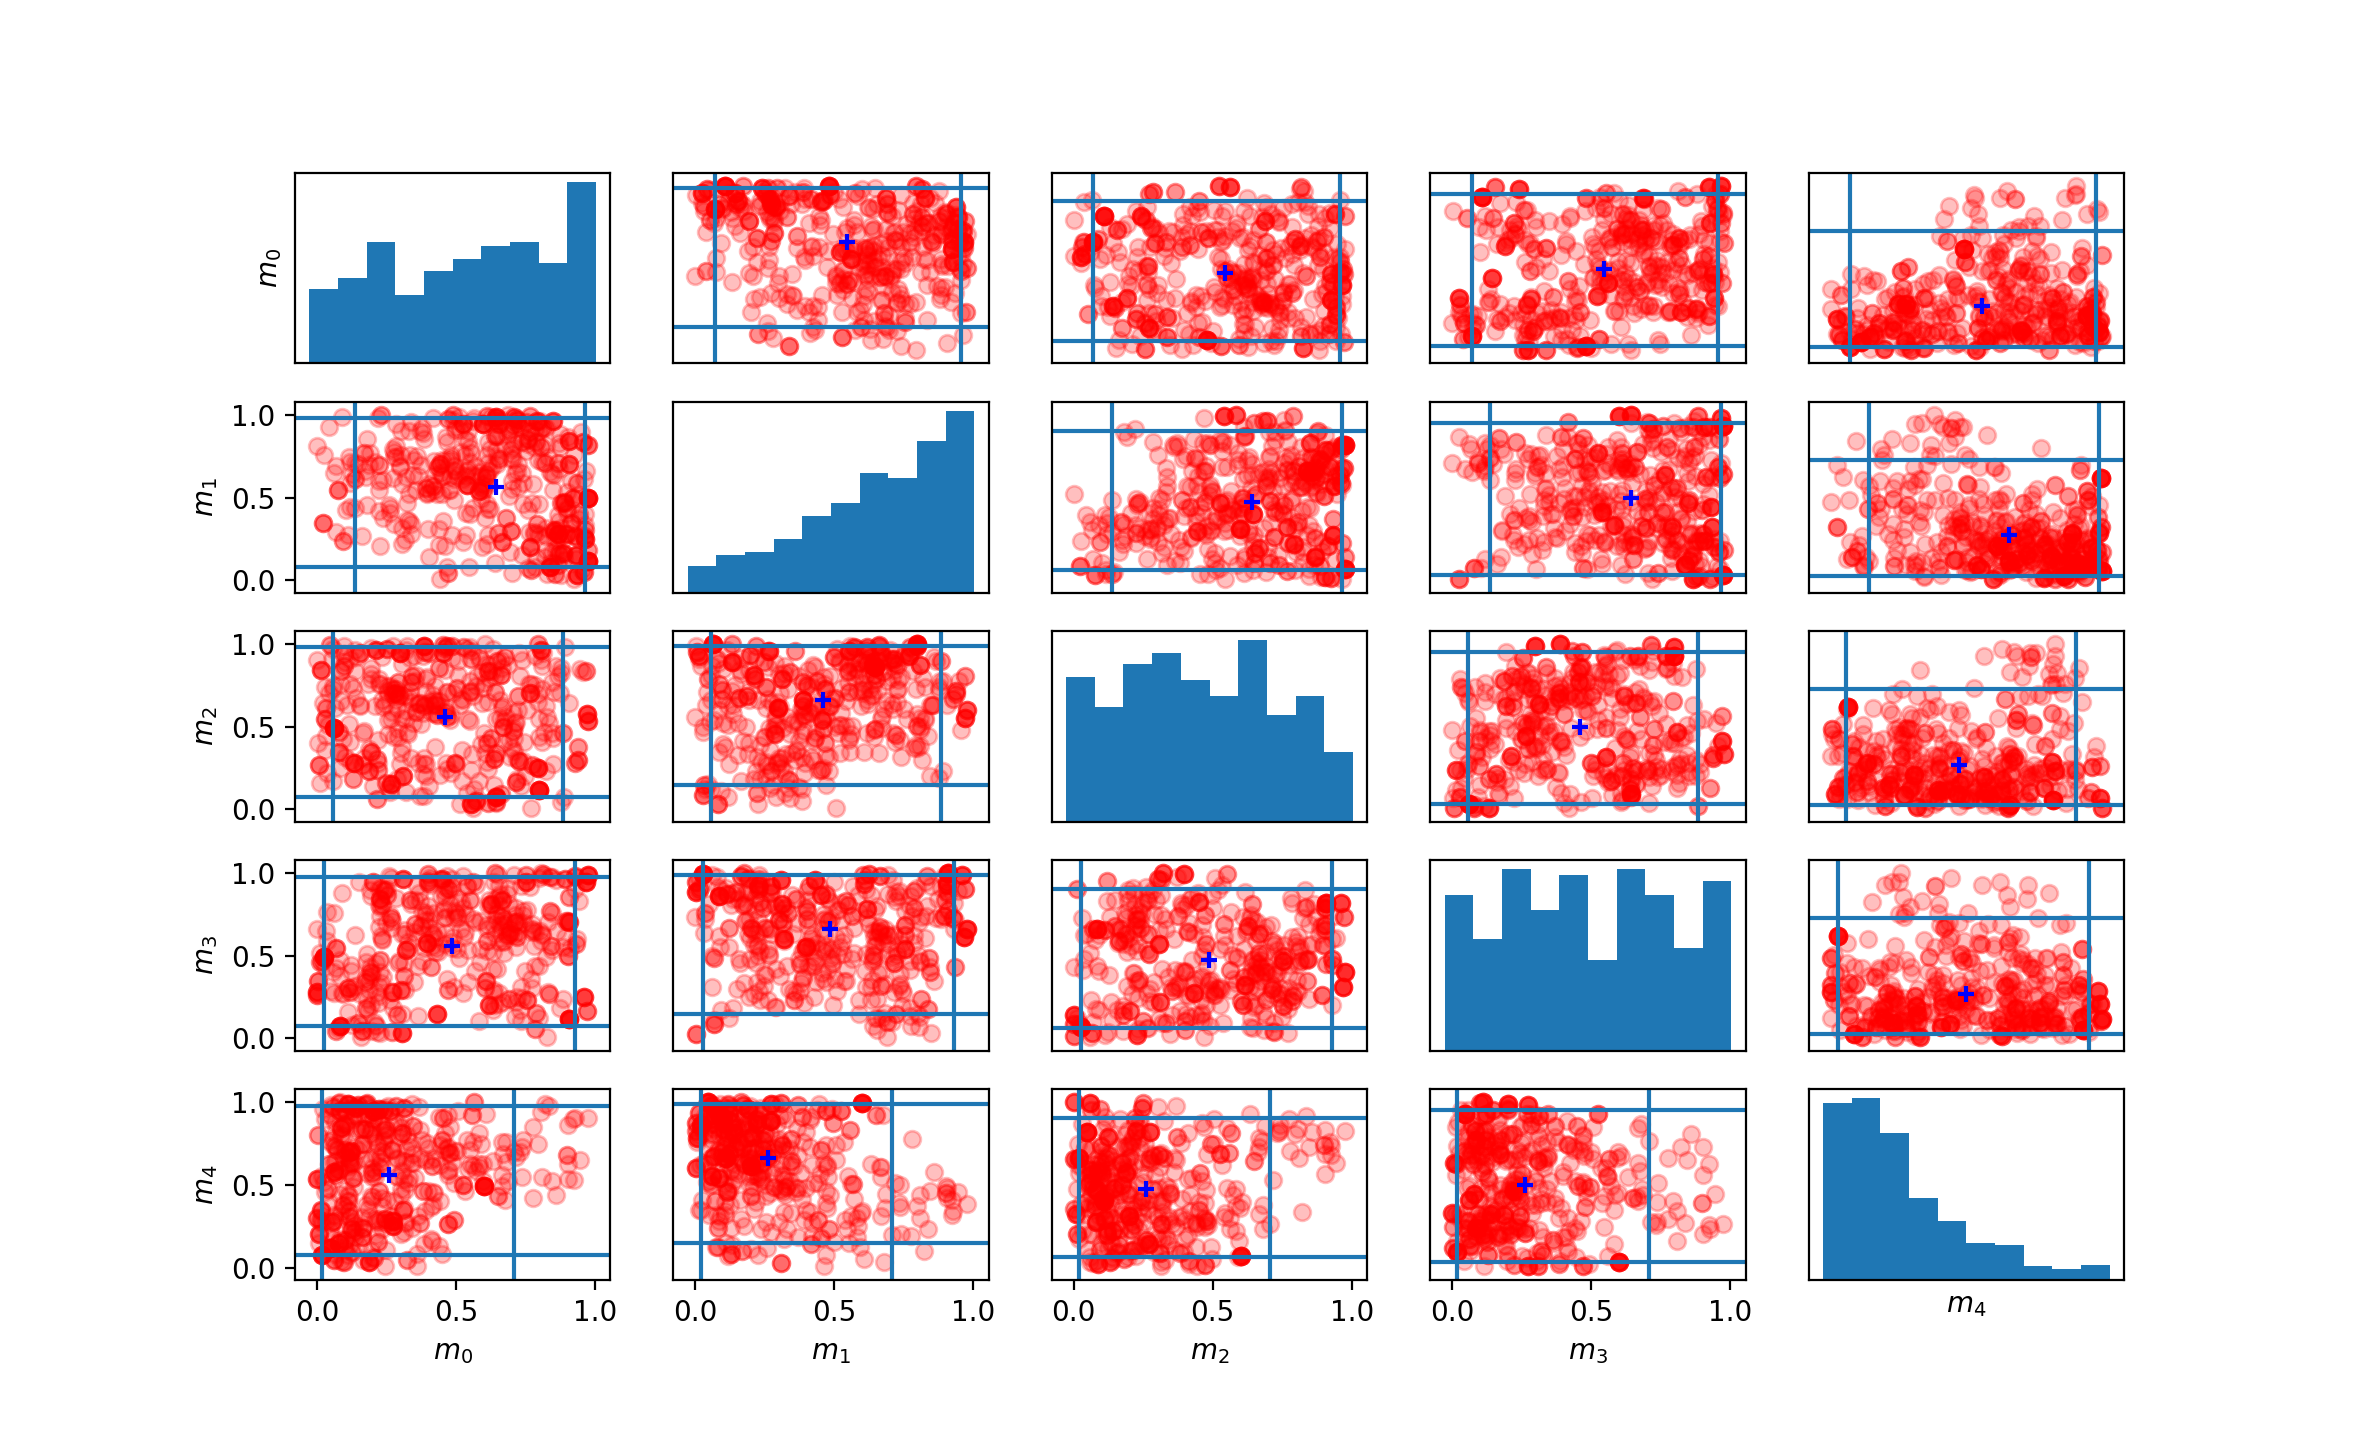
\includegraphics[width=5in]{Fig116.png}
    \caption{Sampled Posterior distributions. The blue squares are the MAP estimate. The 95\% probability intervals are given by the blue lines around each parameter estimate.}
    \label{p1_post_dist}
\end{figure}



\FloatBarrier


\section*{Part 2}
\subsection*{Part a}

It was assumed that all parameters have the same standard deviation of 0.1.

The normal logprior function allows parameter estimates that are within 5 standard deviations from the mean. The log normal probability distribution is calculated as
$$ 
\frac{1}{x \sigma \sqrt{2 \pi}} \exp \left(-\frac{(\ln x-\mu)^{2}}{2 \sigma^{2}}\right)
 $$
 for samples within the 5 $\sigma$ bounds. Values beyond the 5 $\sigma$ support are set to $-\infty$.
\FloatBarrier

\subsection*{Part b}

According to Figure \ref{fig:2b} all five parameters started with a highly positive auto correlation (near one) and rapidly deteriorated to near zero for each parameter after selecting a lag separation of 25,000.
Initially, we started with a lag size of 10,000, however as we estimated the autocorrelation at this distance we felt that increasing the lap distance would improve our sampling. We concluded that a warm up of 100,000 steps is appropriate in our case and the total steps used to sample the posterior distribution was 5,000,000. As shown Figure \ref{fig:2b} the five parameters are highly decorrelated after several steps of 25,000. It appears that a longer burn in period and a greater lag separation should be used to completely decorrelate parameters $\mathbf{m_2},~\mathbf{m_3},~\text{and}~\mathbf{m_5}$.

\begin{figure}[!h]
    \centering
    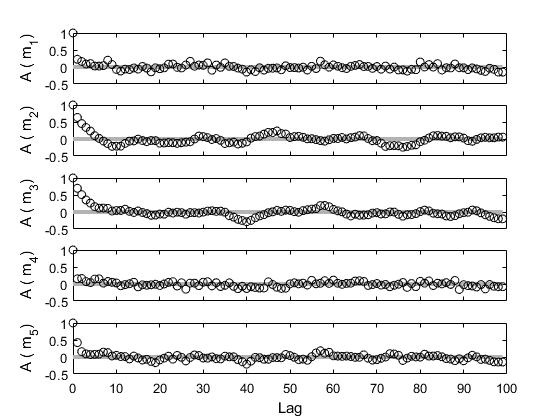
\includegraphics[width=\textwidth]{2b.png}
    \caption{Autocorrelations for posterior distribution parameters after thinning to every $25,000^{th}$ sample.}
    \label{fig:2b}
\end{figure}
\FloatBarrier

\subsection*{Part C}
We present $\sim190$ samples from the posterior distribution after a burn in period and thinning ever $25,000^{th}$ sample. Our assumption of the true parameter estimates is likely inaccurate, as these values are not clearly defined for our soil type. We chose an educated guess as the prior means and a standard deviation of 0.1 for each parameter.

\begin{figure}[!h]
    \centering
    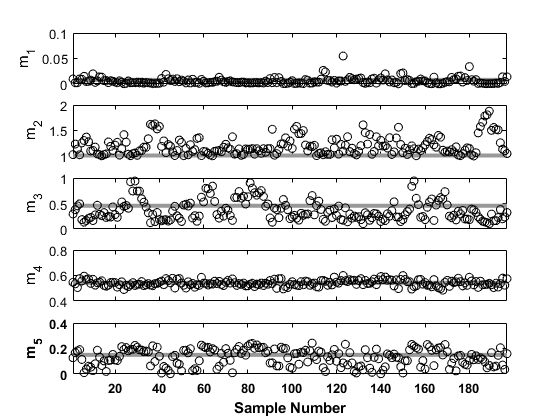
\includegraphics[width=\textwidth]{2c.png}
    \caption{MCMC History of posterior samples. The grey line is the  true parameter estimate which is not well defined for our chosen soil.}
    \label{fig:2c}
\end{figure}
\FloatBarrier


\subsection*{Part D}
Based on the histograms and scatter plots of the resulting sampled posterior distribution shown in Figure \ref{fig:2d}, it can be seen that our parameters estimates of MAP solution and also True model both do lay inside the 95\% probability intervals for every single parameter direction. Despite that, most histograms of the resulting sampled posterior distribution are exponential (i.e. $\mathbf{m_1}$, $\mathnf{m_2}$, $\mathbf{m_3}$) or resembling a uniform distribution ($\mathbf{m_5}$). The van Genuchten problem suffers from non-uniqueness. A variety of combinations of these five parameters can fit the soil data quite well. Using Baysian methods, we impose a probabilistic constraint on the solution space for each parameter based on our knowledge of how these parameters should interact with each other. By doing so we improve the conditioning of the problem. The MCMC technique proved very valuable in acquiring a solution that abides the understood physical bounds of the van Genuchten relationship.

\begin{figure}
    \centering
    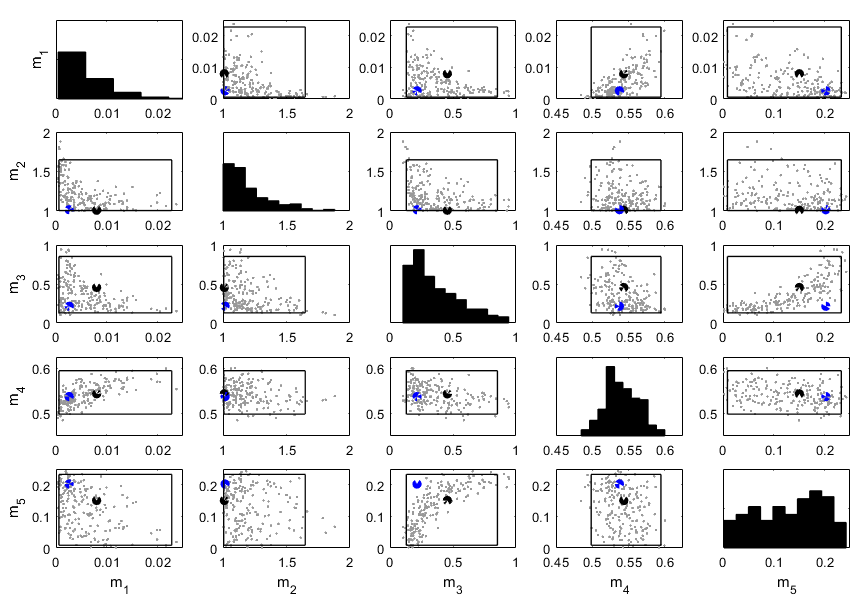
\includegraphics[width=\textwidth]{2d.png}
    \caption{MAP solutions are represented by the blue marker, the ``true" parameter estimates are described by the black marker. $\mathbf{m_4}$ is characterized by a normal distribution though the other parameters do not. This could be the result of our bounds on the prior distribution.}
    \label{fig:2d}
\end{figure}
\FloatBarrier

\subsection*{Part E}
\begin{figure}[!h]
    \centering
    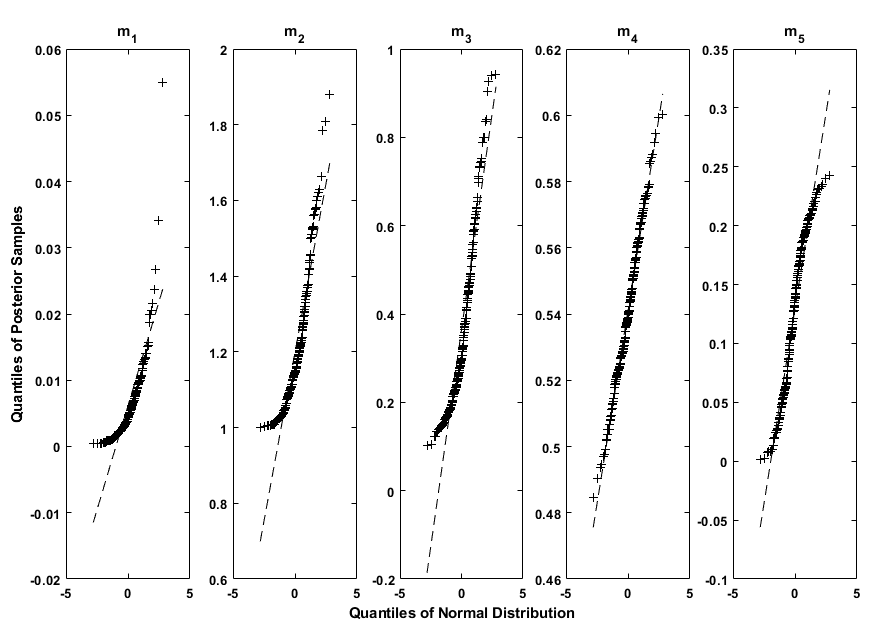
\includegraphics[width = \textwidth]{2e.png}
    \caption{The Quantile-Quantile plots compare the posterior parameter estimate distributions after thinning to a standard normal distribution. $\mathbf{m_4}$ exemplifies normal behavior, however the remaining parameter distributions do not follow the Q-Q line and should not be regarded as normal. }
    \label{fig:2e}
\end{figure}


\newpage
\section{Part1 Code}
\inputminted[]{python}{"main.py"}
\section{Part2 Code}
\inputminted[]{matlab}{"G11.m"}
\inputminted[]{matlab}{"lognormalprior.m"}




\end{document}


